\section{Shika Express Demonstrations for Chemistry}

\begin{multicols}{2}


\subsection{Requirements for Combustion}

\begin{center}
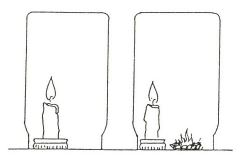
\includegraphics[width=0.4\textwidth]{./img/source/flame-extinguisher.jpg}
\end{center}

\begin{description*}
\item[Topic:]{Combustion - Form I}
\item[Materials:]{2 glass jars, 2 candles, bottle caps, kerosene or spirit}
%\item[Setup:]{}
\item[Procedure:]{Place 1 jar over a lit candle and the other jar over both a candle and a kerosene or spirit flame in a bottle cap.}
%\item[Hazards:]{}
\item[Questions:]{Which candle flame goes out first?}
\item[Observations:]{The candle in the jar with the spirit burner goes out first.}
\item[Theory:]{Three elements are necessary for combustion: heat, fuel and oxygen. In the second jar, both the candle and spirit flame are consuming oxygen and so the oxygen gets depleted faster, extinguishing the flame.}
%\item[Applications:]{}
%\item[Notes:]{}
\end{description*}

\subsection{Constructing a Water Filter}

\begin{center}
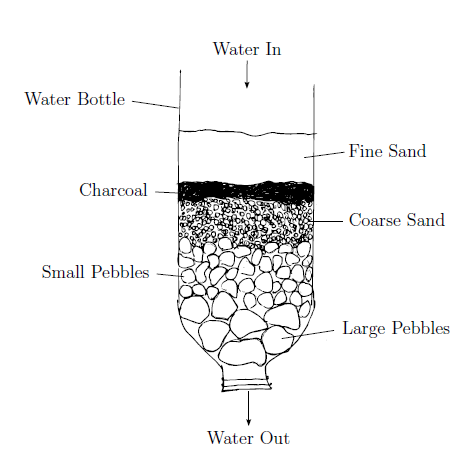
\includegraphics[width=0.4\textwidth]{./img/water-filter.png}
\end{center}

\begin{description*}
\item[Topic:]{Water - Form II}
\item[Materials:]{Fine sand, coarse sand, small pebbles, large pebbles, charcoal, empty bottle, dirty water}
\item[Setup:]{Rinse off all pebbles and remove and dirt from the sand. Cut the bottom of a bottle so it is shaped like a funnel.}
\item[Procedure:]{Invert the bottle and place the large pebbles, followed by smaller pebbles, coarse sand, charcoal and sand on top. Run water through until it comes out clean on bottom.}
%\item[Hazards:]{}
%\item[Questions:]{}
%\item[Observations:]{}
\item[Theory:]{When dirty water passes through sand particles, impurities are trapped and
remain above. The smallest particles and some micro-organisms are stopped
by the charcoal layer.}
%\item[Applications:]{}
%\item[Notes:]{}
\end{description*}

\subsection{The `SODIS' Method} % PIC!!!

%\begin{center}
%\includegraphics[width=0.4\textwidth]{./img/.jpg}
%\end{center}

\begin{description*}
\item[Topic:]{Water - Form II}
%\item[Materials:]{}
%\item[Setup:]{}
\item[Procedure:]{Fill a bottle with water from a tap. Place it on the roof of your house in open sunlight for 2 days or 3-4 days if it is cloudy. Filter through a clean cloth or kanga.}
%\item[Hazards:]{}
%\item[Questions:]{}
%\item[Observations:]{}
\item[Theory:]{Ultraviolet rays from the sun kill the harmful bacteria in the water that cause disease. Filtering though a cloth removes solid impurities.}
%\item[Applications:]{}
%\item[Notes:]{}
\end{description*}

\subsection{Arranging Shapes}

\begin{center}
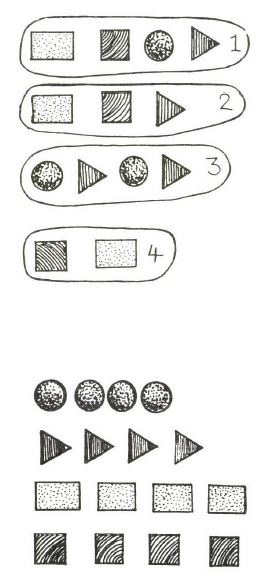
\includegraphics[width=0.4\textwidth]{./img/source/arranging-shapes.jpg}
\end{center}

\begin{description*}
\item[Topic:]{Periodic Classification - Form II}
\item[Materials:]{Paper/manila or card, scissors, coloured pencils or markers}
%\item[Setup:]{}
\item[Procedure:]{Make several of each of the following
shapes: squares (3 $\times$ 3 cm), triangles (3 cm sides),
rectangles (3 $\times$ 4 cm), circles (3 cm diameter). Make some of the same shape which are smaller and larger than these as well. Colour them all differently (not according to shape).
Mix the shapes and then sort them according to
a chosen feature. }
%\item[Hazards:]{}
\item[Questions:]{How many different ways can
you find of grouping the shapes?}
%\item[Observations:]{}
%\item[Theory:]{}
%\item[Applications:]{}
%\item[Notes:]{}
\end{description*}

\subsection{Models of Atoms}

\begin{center}
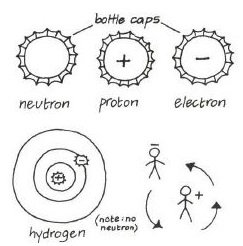
\includegraphics[width=0.4\textwidth]{./img/vso/atom-model.jpg}
\end{center}

\begin{description*}
\item[Topic:]{Atomic Structure - Form II}
\item[Materials:]{Bottle caps, marker}
%\item[Setup:]{}
\item[Procedure:]{Label bottle caps at protons (`+'), electrons (`-') and neutrons (blank). Create models for different atoms by placing the appropriate number of protons and neutrons in the center (nucleus) and electrons on drawn circles around the outside. Draw circles on desks or
floors to represent the electron
shells. }
%\item[Hazards:]{}
%\item[Questions:]{}
%\item[Observations:]{}
\item[Theory:]{All atoms contain a nucleus
(protons and neutrons) and
electrons found in different shells around the nucleus. }
%\item[Applications:]{}
\item[Notes:]{Alternatively use students
to represent the electron shells.}
\end{description*}

\subsection{$\mathrm{CO_2}$ Balloon}

\begin{center}
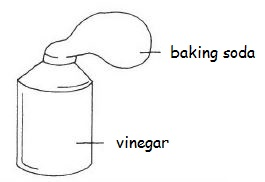
\includegraphics[width=0.4\textwidth]{./img/vso/co2-balloon.jpg}
\end{center}

\begin{description*}
\item[Topic:]{Acid and Bases - Form III}
\item[Materials:]{Bottle, baking soda, vinegar, balloon}
%\item[Setup:]{}
\item[Procedure:]{Add a small amount of vinegar into a bottle. Fill a balloon with baking soda (bicarbonate of soda) and stretch the balloon over the mouth of the bottle. Lift the balloon to empty the contents into the bottle.}
%\item[Hazards:]{}
%\item[Questions:]{}
\item[Observations:]{The balloon fills up with gas and may even explode!}
\item[Theory:]{The vinegar (acid) and baking soda (base) combine to produce carbon dioxide gas, which gets collected in the balloon.}
%\item[Applications:]{}
%\item[Notes:]{}
\end{description*}

\subsection{Molecule Models} % Source 114

\begin{center}
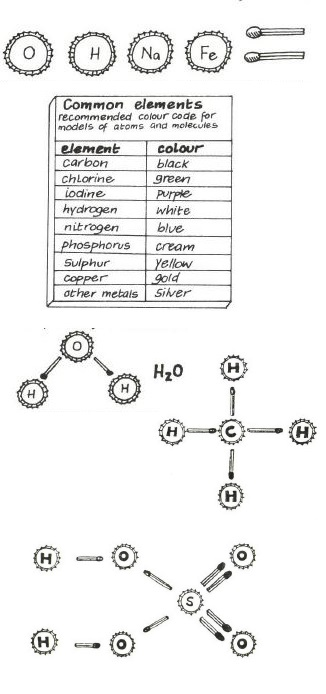
\includegraphics[width=0.4\textwidth]{./img/vso/molecule-model.jpg}
\end{center}

\begin{description*}
\item[Topic:]{Chemical Formula - Form II}
\item[Materials:]{Bottle caps, matches}
%\item[Setup:]{}
\item[Procedure:]{Mark the bottle caps with a pen or marker. Matchsticks form the bonds. Colour the bottle caps according to the recommendations given to represent different elements. Try to make all the examples in your textbook.}
%\item[Hazards:]{}
%\item[Questions:]{}
%\item[Observations:]{}
%\item[Theory:]{}
%\item[Applications:]{}
%\item[Notes:]{}
\end{description*}

\subsection{Rosella Indicator}

\begin{center}
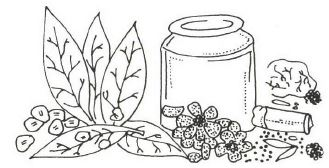
\includegraphics[width=0.4\textwidth]{./img/vso/making-indicators.jpg}
\end{center}

\begin{description*}
\item[Topic:]{Acid and Bases - Form III}
\item[Materials:]{Rosella leaves, paper, straw, hot water, lemon or vinegar, bicarbonate of soda}
\item[Setup:]{Prepare an indicator solution from rosella leaves by crushing and adding to boiled water.}
\item[Procedure:]{Place a small amount of vinegar or lemon juice to one bottle cap and some bicarbonate of soda to another. Add a few drops of indicator to each cap, noting any colour changes that occur.}
%\item[Hazards:]{}
%\item[Questions:]{}
%\item[Observations:]{}
\item[Theory:]{The vinegar should turn a reddish colour, indicating it is acidic. The bicarbonate of soda a greenish or blue colour, indicating it is a basic.}
%\item[Applications:]{}
\item[Notes:]{Dip thin strips of paper in the indicator solution and let dry to make home-made litmus paper.}
\end{description*}

\end{multicols}
